\documentclass[border=3pt]{standalone}
% Shared preamble for the standalone figures.
\usepackage[T1]{fontenc}
\usepackage[scaled=0.9]{helvet}
\renewcommand{\familydefault}{\sfdefault}
\usepackage{tikz}
\usetikzlibrary{arrows.meta,positioning,calc}

\definecolor{ink}{RGB}{28,28,30}
\definecolor{rule}{RGB}{95,97,104}
\definecolor{muted}{RGB}{112,114,121}
\definecolor{accent}{RGB}{172,56,44}
\definecolor{probfill}{RGB}{250,244,235}
\definecolor{detfill}{RGB}{239,243,247}

\newcommand{\zone}[1]{{\fontsize{6.6}{8}\selectfont\bfseries #1}}
\newcommand{\sub}[1]{{\fontsize{7.2}{9}\selectfont\color{muted}#1}}
\newcommand{\mono}[1]{{\fontencoding{OT1}\fontfamily{cmtt}\selectfont #1}}

\tikzset{
  every picture/.style={font=\fontsize{8}{10}\selectfont, text=ink,
    >={Stealth[length=4.6pt,width=3.8pt]}},
  box/.style={draw=rule, line width=0.5pt, rounded corners=2pt, fill=white,
    minimum height=8mm, minimum width=16mm, inner sep=2pt, align=center},
  flow/.style={->, draw=rule, line width=0.6pt},
  hot/.style={->, draw=accent, line width=0.9pt},
  lbl/.style={font=\fontsize{7.2}{9}\selectfont, text=muted, inner sep=1.5pt},
}

\begin{document}
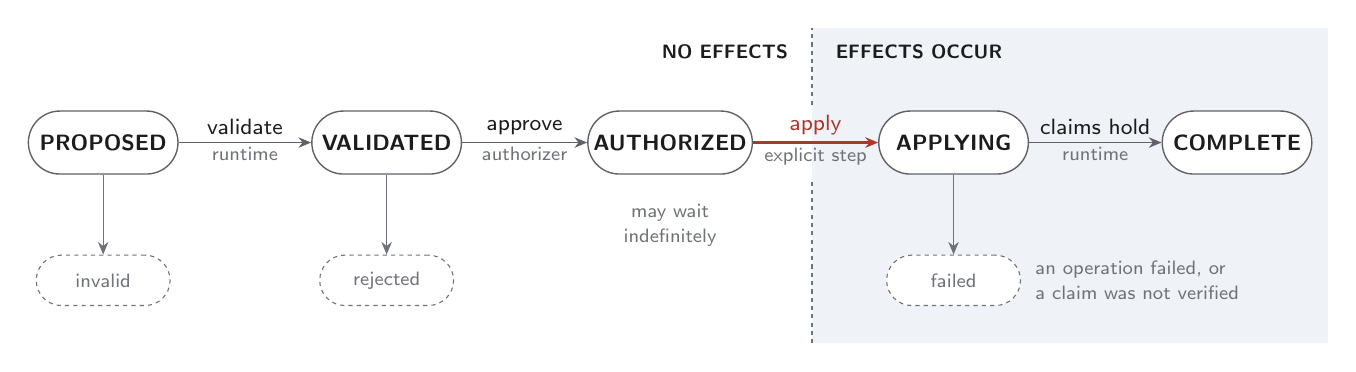
\begin{tikzpicture}
\tikzset{
  state/.style={draw=rule, line width=0.5pt, rounded corners=4mm, fill=white,
    minimum height=8mm, minimum width=19mm, inner sep=2pt, align=center,
    font=\fontsize{7.6}{9}\selectfont\bfseries},
  term/.style={draw=muted, line width=0.4pt, dash pattern=on 1.5pt off 1.5pt,
    rounded corners=3.2mm, fill=white, minimum height=6.4mm, minimum width=17mm,
    inner sep=2pt, align=center, font=\fontsize{7.2}{9}\selectfont, text=muted},
  act/.style={font=\fontsize{7.6}{9}\selectfont, inner sep=2.5pt},
}

% effects region
\fill[detfill] (9.0,-2.55) rectangle (15.55,1.45);
\node[anchor=west] at (9.18,1.15) {\zone{EFFECTS OCCUR}};
\node[anchor=east] at (8.82,1.15) {\zone{NO EFFECTS}};
\draw[muted, line width=0.5pt, dash pattern=on 1.5pt off 1.5pt] (9.0,-2.55) -- (9.0,-0.5) (9.0,0.48) -- (9.0,1.45);

\node[state] (p) at (0,0)    {PROPOSED};
\node[state] (v) at (3.6,0) {VALIDATED};
\node[state] (a) at (7.2,0)  {AUTHORIZED};
\node[state] (x) at (10.8,0){APPLYING};
\node[state] (d) at (14.4,0) {COMPLETE};

\draw[flow] (p) -- node[above, act] {validate} node[below, lbl] {runtime} (v);
\draw[flow] (v) -- node[above, act] {approve} node[below, lbl] {authorizer} (a);
\draw[hot]  (a) -- node[above, act, text=accent] {apply} node[below, lbl] {explicit step} (x);
\draw[flow] (x) -- node[above, act] {claims hold} node[below, lbl] {runtime} (d);

\node[term] (ti) at (0,-1.75)     {invalid};
\node[term] (tr) at (3.6,-1.75)  {rejected};
\node[term] (tf) at (10.8,-1.75) {failed};
\draw[flow, draw=muted, line width=0.45pt] (p) -- (ti);
\draw[flow, draw=muted, line width=0.45pt] (v) -- (tr);
\draw[flow, draw=muted, line width=0.45pt] (x) -- (tf);

\node[lbl, align=center] at (7.2,-1.05) {may wait\\indefinitely};
\node[lbl, anchor=west, align=left] at (11.78,-1.75) {an operation failed, or\\a claim was not verified};
\end{tikzpicture}
\end{document}
